% AI POWERED COCONUT HARVESTING SYSTEM - IRJMETS-style paper (LaTeX)
% Fonts: Cambria (headings/title) + Times New Roman (body), matching paper/IRJMETSTemplate.docx
% Compile: tectonic main.tex
\documentclass[10pt,a4paper]{article}

\usepackage{fontspec}
\usepackage{geometry}
\usepackage{graphicx}
\usepackage{url}
\usepackage{array}
\usepackage{float}
\usepackage{placeins}
\usepackage{needspace}
\usepackage{etoolbox}

% Suppress the environment's own "References" heading (the \irjsec heading is used instead)
\patchcmd{\thebibliography}{\section*{\refname}}{}{}{}

\geometry{top=2.09in,bottom=0.85in,left=0.83in,right=0.83in,headheight=140.6426pt,headsep=10pt,footskip=0.38in}

% Cambria from Microsoft Office bundled fonts
\newfontfamily\cambria[
  Path=/Applications/Microsoft Excel.app/Contents/Resources/DFonts/,
  BoldFont={Cambriab.ttf},ItalicFont={Cambriai.ttf},BoldItalicFont={Cambriaz.ttf}
]{Cambria.ttc}

% Times New Roman system font
\setmainfont[
  Path=/System/Library/Fonts/Supplemental/,
  BoldFont={Times New Roman Bold.ttf},ItalicFont={Times New Roman Italic.ttf},
  BoldItalicFont={Times New Roman Bold Italic.ttf}
]{Times New Roman.ttf}

\setlength{\parindent}{0pt}
\setlength{\parskip}{3pt}

% IRJMETS-style headings
\newcommand{\irjsec}[1]{\par\vspace{6pt}\noindent{\cambria\bfseries\fontsize{12}{14}\selectfont\textbullet~#1}\par\vspace{3pt}}
\newcommand{\irjsub}[1]{\par\vspace{4pt}\noindent{\cambria\bfseries\fontsize{10}{12}\selectfont #1}\par\vspace{2pt}}

% Caption helpers (IRJMETS: figure captions below, table captions above)
\newcommand{\tablecap}[1]{\par\vspace{6pt}\begin{center}{\cambria\bfseries\fontsize{10}{12}\selectfont #1}\end{center}\vspace{-2pt}}
\newcommand{\figcap}[1]{\par\vspace{2pt}\begin{center}{\fontsize{9}{11}\selectfont #1}\end{center}}

% ---------- IRJMETS running header/footer (template header2/footer2) ----------
\usepackage{xcolor}
\definecolor{irjgreen}{HTML}{00B050}  % journal name, e-ISSN, footer URL
\definecolor{irjlink}{HTML}{0000FF}   % footer URL hyperlink
\definecolor{irjnavy}{HTML}{1F497D}   % subtitle + volume/impact line
\definecolor{irjslate}{HTML}{44546A}  % page number

\usepackage{fancyhdr}
\pagestyle{fancy}
\fancyhf{}
\renewcommand{\headrulewidth}{0.4pt}
\renewcommand{\footrulewidth}{0.4pt}

\fancyhead[C]{%
\vbox{%
\hbox to \textwidth{\hfil
\includegraphics[height=0.9in]{figures/extracted/image6.png}\hfil}%
\kern3pt
\hbox to \textwidth{\hfil{\color{irjgreen}\bfseries\fontsize{12}{14}\selectfont e-ISSN: 2582-5208}}%
\kern3pt
\hbox to \textwidth{\hfil{\color{irjgreen}\bfseries\fontsize{12.5}{14}\selectfont International Research Journal of Modernization in Engineering Technology~ and~ Science}\hfill}%
\kern3pt
\hbox to \textwidth{\hfil{\color{irjnavy}\bfseries\fontsize{12}{14}\selectfont ( Peer-Reviewed, Open Access, Fully Refereed International Journal )}\hfil}%
\kern3pt
\hbox to \textwidth{\color{irjnavy}\bfseries\fontsize{12}{14}\selectfont Volume:08/Issue:03/March-2026\hfill Impact Factor- 8.187\hfill www.irjmets.com}%
}}

\fancyfoot[C]{%
\vbox{%
\hbox to \textwidth{{\color{irjlink}\fontsize{9}{11}\selectfont\underline{www.irjmets.com}}\hfill{\color{irjgreen}\fontsize{9}{11}\selectfont @International Research Journal of Modernization in Engineering, Technology and Science}}%
\kern2pt
\makebox[\textwidth][c]{\color{irjslate}[\thepage]}%
}}

\begin{document}

% ---------- Title block ----------
\begin{center}
{\cambria\bfseries\fontsize{14}{17}\selectfont AI POWERED COCONUT HARVESTING SYSTEM}\\[10pt]
{\cambria\bfseries\fontsize{12}{14}\selectfont
Dr.~Madhu B.K\textsuperscript{*1}, Mahesh S\textsuperscript{*2}, Syeda Umme Haani\textsuperscript{*3}, S Mohammed Maaz\textsuperscript{*4}, Akshatha G\textsuperscript{*5}}\\[6pt]
{\cambria\fontsize{11}{13}\selectfont
\textsuperscript{1}Dean \& Professor, Department of Computer Science and Engineering, Vidya Vikas Institute of Engineering and Technology, Mysuru, Karnataka, India.}\\[2pt]
{\cambria\fontsize{11}{13}\selectfont
\textsuperscript{2,3,4,5} Final-year B.E. Students, Department of Computer Science and Engineering, Vidya Vikas Institute of Engineering and Technology, Mysuru, Karnataka, India.}
\end{center}

\vspace{2pt}
\noindent{\cambria\bfseries ABSTRACT}\\[2pt]
Manual coconut harvesting depends on climbers working at heights of 15 to 25 metres, and growers have no digital record of which trees are ready to harvest. This paper presents an AI powered coconut harvesting system (Veraxis), a full-stack digital twin platform that turns drone survey imagery into a structured, queryable plantation model and drives a simulated climbing robot to harvest it. A YOLOv8 tree detector processes survey tiles laid out by a configurable flight planner; GPS-proximity matching with a 4 m radius assigns permanent tree identities and mission-scoped observations; a second YOLOv8 model classifies close-up coconuts as Mature, Potential or Premature and writes immutable inventory snapshots; and a nearest-neighbour planner builds immutable harvest missions. The robot is a deterministic, event-driven simulation with a frozen state machine, battery model and WebSocket telemetry, so real hardware would replace only the engine. The contribution is the integration rather than any new network or learning rule: a digital twin that keeps a plantation as a persistent, queryable object and evaluates the complete workflow, from survey tiles to a finished harvest, end to end. In our tests the engine reproduced identical traces in 100 of 100 randomised missions with no illegal state transition, nearest-neighbour routes were 5.6 to 9.2 percent longer than optimal for 5 to 8 trees, and re-survey matching created no duplicate trees for position errors up to about 1 m. The robot remains simulated and field trials are future work.\\[4pt]
\noindent{\bfseries Keywords}: Digital Twin, Precision Agriculture, Coconut Harvesting, YOLOv8, Robot Simulation, WebSocket Telemetry

% ================= INTRODUCTION =================
\irjsec{INTRODUCTION}
Coconut is a major plantation crop, yet harvesting it has changed little in decades. The dominant method is a human climber carrying a knife up an unprotected trunk, which is physically dangerous and increasingly hard to staff because fewer young workers are willing to take up the work. A second problem is informational: plantations are usually run from memory or paper, with no canonical list of trees, no position for each, no fruit count per tree and no record of past harvests. The grower therefore cannot easily answer the central economic question of which trees are worth visiting now.

This work addresses both problems with one system, named Veraxis. Its key design decision is to split sensing between two actors with different strengths. A drone gives cheap, wide-area, top-down coverage and is used only to find and locate trees. A climbing robot gives close-up views of the canopy and is used to judge ripeness, which a top-down view from altitude cannot do reliably. Keeping the two tasks in two separate detectors lets each model be retrained or replaced without touching the other.

The contribution of this work is not a new detection algorithm, loss function or network architecture: the detectors are standard YOLOv8 models, and the routing heuristic and state-machine pattern are established techniques. The contribution is the integration itself: a digital twin architecture that combines YOLOv8-based perception with autonomous mission planning and evaluates the full harvesting workflow end to end, treating the plantation as a persistent, queryable object rather than a one-off detection result.

The main contributions of this work are:
\begin{itemize}
\itemsep1pt
\item \textbf{Development of a digital twin platform} for autonomous coconut harvesting that keeps the plantation as a persistent, queryable object rather than a one-off detection result. The platform includes permanent tree identities built from GPS-proximity matching (a 4 m Haversine radius) with a mission-scoped observation history, a farm-pixel twin viewer that shares one coordinate function between the tile mosaic, tree overlay and robot layer, and immutable inventory snapshots and harvest missions.
\item \textbf{Integration of YOLOv8-based real-time perception} into the platform. A one-class tree detector processes drone survey tiles, a three-class ripeness classifier (Mature, Potential, Premature) processes close-up images, and both use the lightweight YOLOv8n network with its anchor-free decoupled head and C2f-style feature fusion [2], so each detector can be retrained or replaced without touching the other.
\item \textbf{Evaluation of the complete harvesting workflow} under reproducible simulated harvesting scenarios: a full pipeline run from survey tiles to a finished harvest, deterministic replay of the simulated engine over 100 randomised missions (identical traces in 100 of 100), and exhaustive legality checks of all 64 ordered state-machine transitions.
\item \textbf{Analysis of detection accuracy and operational efficiency:} precision, recall and mAP on held-out validation splits with an interpretation of the per-class error structure, routing quality of the nearest-neighbour planner against exact-optimal and 2-opt references (5 to 100 trees), matching resilience under re-survey position error, and engine throughput.
\end{itemize}

% ================= RELATED WORK =================
\irjsec{RELATED WORK}
Single-stage detectors in the YOLO family frame detection as one regression problem and run in real time [1], and the Ultralytics YOLOv8 implementation [2] is widely used for agricultural targets. Fruit detection in orchards with deep networks has been studied for crops such as mango and other tree fruit [3], [4]; those systems concentrate on counting and yield estimation from imagery rather than on closing the loop to a harvesting actor. The digital twin idea, a persistent virtual counterpart of a physical asset that is kept in step with it [5], motivates our choice to make the plantation a permanent, queryable object instead of a one-off detection result.

On the planning side, ordering a set of stops to minimise travel is the travelling salesman problem. The nearest-neighbour heuristic is simple and fast but not optimal, and its worst-case behaviour has been analysed [6]; two-exchange (2-opt) local search [7] is a standard way to obtain a stronger reference tour. For control, we model the robot as a finite state machine in the spirit of statecharts [8], and we stream its state to clients with the WebSocket protocol [9] so that live position does not require polling.

% ================= SYSTEM ARCHITECTURE =================
\irjsec{SYSTEM ARCHITECTURE}
Veraxis has three layers: a Next.js and React frontend that only presents data, a FastAPI backend that owns all business rules, and PostgreSQL storage accessed through SQLAlchemy. The machine-learning models run locally inside the backend. Fig.~1 shows the end-to-end flow from survey to harvest. The backend is the single source of truth and the frontend never computes business results, which keeps eligibility, planning and state transitions in one place.

\begin{figure}[!ht]
\centering
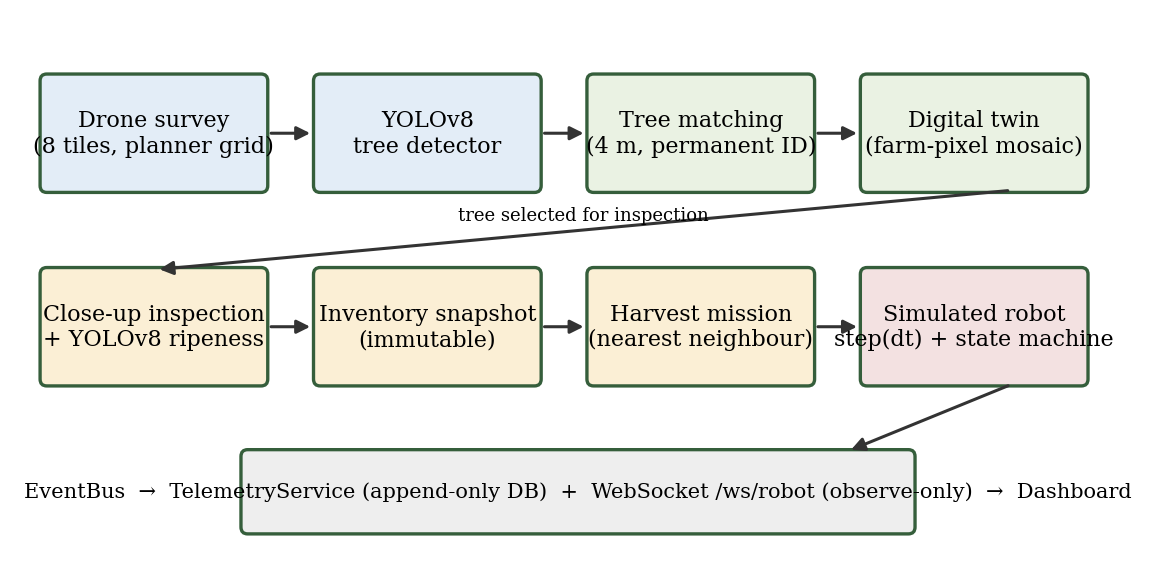
\includegraphics[width=0.8\textwidth]{figures/extracted/image1.png}
\figcap{Figure 1: End-to-end pipeline and telemetry path. Splitting perception (drone survey tiles) from inspection (robot close-ups) into separate stages is what lets either detector be retrained or replaced independently.}
\end{figure}

The robot subsystem is deliberately split into three concerns. Route planning (which trees, in what order) belongs to the harvest planner. Movement planning (the farm-pixel trajectory between stops) belongs to a pure, stateless navigator. Execution (advancing time, updating position, battery and state) belongs to the simulation engine and its scheduler, the only components that mutate live robot state. Because the contract with the outside world is the HTTP command set plus the WebSocket telemetry frame, a physical robot could replace the simulation engine and leave every other component unchanged.

% ================= METHODOLOGY =================
\irjsec{METHODOLOGY}
\irjsub{A. Survey ingestion and flight planning}
A survey mission is created from a folder of drone images. A simulated Flight Planner owns the coverage geometry through an explicit configuration (rows, columns, origin corner, traversal pattern and row/column spacing). The grid is never inferred from the number of images: fewer images than planned positions leave positions empty, and more images than positions raise a validation error (HTTP 422). Positions are visited in boustrophedon (lawnmower) order, and each position stores its grid row and column, capture order and image size on the survey tile. Our demonstration survey uses eight tiles in a $2\times4$ grid.

\irjsub{B. Tree detection}
Each tile is passed to a YOLOv8 tree detector with a single class and an inference confidence threshold of 0.4. Detections are stored as raw bounding boxes per tile. They are not trees yet: a detection becomes a tree only after matching.

\irjsub{C. Permanent tree identity}
A detection's GPS position is generated from the mission base coordinate, the tile's grid position and the box centre offset, using a ground scale derived from the tile footprint (a spacing of 0.001 degrees, about 111 m, so roughly 0.054 m per pixel for a 2048-pixel tile). Matching uses the Haversine distance: a detection within 4 m of an existing tree reuses it, otherwise a new tree is created with a write-once identifier (TREE-0001, TREE-0002, ...). A hybrid score weights GPS proximity at 0.7 and bounding-box geometry at 0.3 to choose between candidates. Every detection is also stored as a TreeObservation holding the tile, the pixel position, the bounding box and the confidence. Observations are mission-scoped and never overwritten, and each tree points to one representative observation chosen by a fixed rule: highest confidence, then closest to the tile centre, then newest mission.

\irjsub{D. Digital twin and farm-pixel coordinates}
The twin lays tiles out by their persisted grid row and column in a continuous mosaic with a small configurable seam gap (Fig.~2). It does not stitch or warp images. A single function computes the farm-pixel position of every tile, and the tree overlay and the robot layer use the same function, so a tree box and the robot marker always agree. GPS remains backend metadata. The viewer uses Pointer Events for pan and pinch zoom, viewport culling and zoom-dependent detail, and selecting a tree opens a read-only details drawer.

\begin{figure}[!ht]
\centering
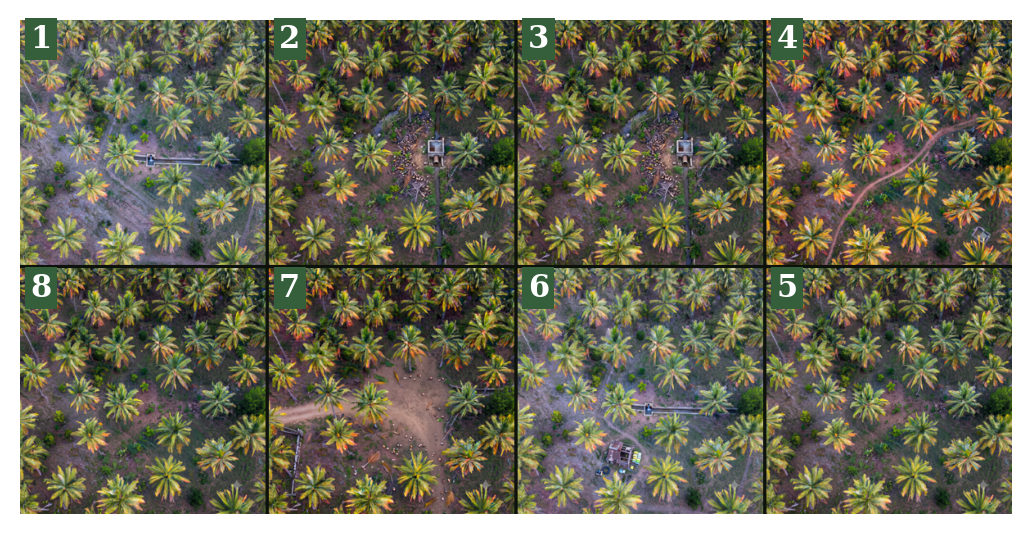
\includegraphics[width=0.95\textwidth]{figures/extracted/image2.png}
\figcap{Figure 2: Farm mosaic of the eight demonstration survey tiles in boustrophedon capture order (numbers 1 to 8). Tiles are placed from persisted grid coordinates rather than stitched, so the same coordinate function grounds the tree overlay and the robot layer exactly as shown.}
\end{figure}

\irjsub{E. Ripeness inspection and inventory}
For one tree, close-up images are uploaded as an inspection session and passed to a second YOLOv8 model with three classes (Mature, Potential, Premature) and a confidence threshold of 0.25. Labels are stored in lowercase and aggregated by a direct group-by into an InventorySnapshot with total, mature, potential and premature counts. A snapshot is immutable and unique per inspection. A new scan creates a new snapshot and repoints the tree's current-inventory pointer, so inventory is replaced on every scan, never accumulated, and history is preserved.

\irjsub{F. Harvest planning}
The planner reads each tree's latest snapshot and selects trees that are active, have an inventory and contain at least one coconut of the requested type (mature, potential, premature or all). Trees already in a live mission are excluded. Selected trees are ordered by nearest neighbour starting from the depot, with candidates processed in ascending tree-id order and ties resolved by a strict comparison, so the order is reproducible. The result is an immutable harvest mission with one item per tree and a unique constraint that prevents a tree from appearing twice.

\irjsub{G. Robot simulation, state machine and telemetry}
The simulation engine advances a context by one fixed step through a pure function, step(dt), with no clock, database or randomness. Movement is linear interpolation between waypoints in farm-pixel space. At each tree the robot climbs (2 s), scans (2 s) and harvests (3 s) in simulated time, then moves on; at the end it returns to the dock. Battery drains only in active states at 1/60 percent per simulated second, which gives about 1 percent per real second at the default $60\times$ speed, and when the level reaches the low threshold (20 percent by default) the engine diverts to the dock.

Robot status is held in eight states (Idle, Moving, Climbing, Scanning, Harvesting, Returning, Error, Docked). A state machine with a frozen transition table is the only component allowed to change the persisted status; every operational state may fault into Error, and Error may recover only to Returning or Idle (Fig.~3). The scheduler drives the engine against wall-clock time at a configurable speed factor and publishes each tick's events to an event bus. A telemetry service appends one telemetry row per tick and one event row per event, and a WebSocket gateway broadcasts the same frames to any number of observe-only clients. When a run ends, one summary record is written with distance, battery use, recharge count, harvest timing and a deterministic mission score equal to $100\times$completion$\times(0.5+0.5\times$battery economy$)\times$a status factor (1.0 completed, 0.5 aborted, 0.2 failed).

\begin{figure}[!ht]
\centering
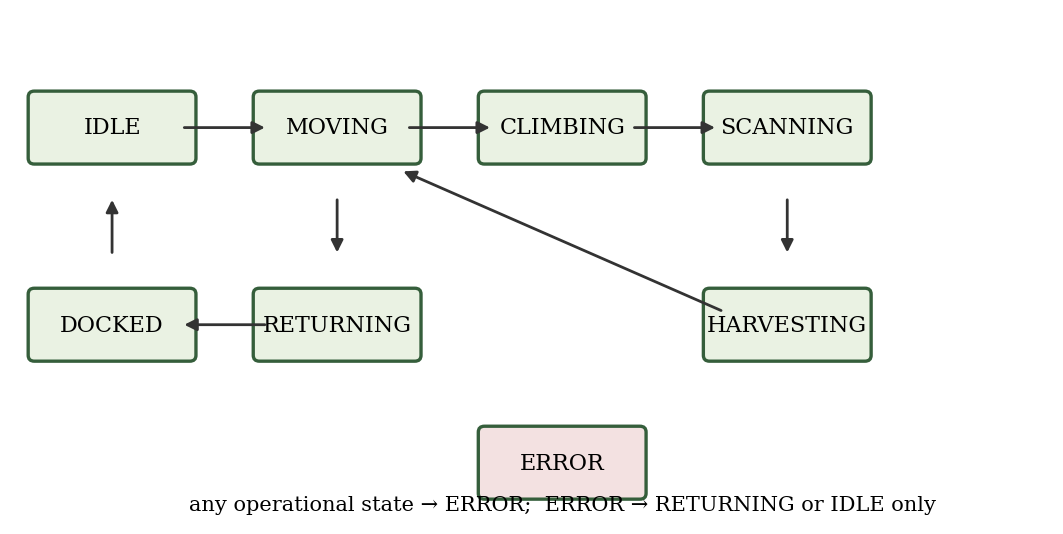
\includegraphics[width=0.7\textwidth]{figures/extracted/image3.png}
\figcap{Figure 3: Robot state machine with the frozen legal transitions. The state machine is the only component that may change robot status: every operational state can fault into Error, and Error recovers only to Returning or Idle, so no run can enter an undefined state.}
\end{figure}

% ================= EXPERIMENTAL SETUP =================
\irjsec{EXPERIMENTAL SETUP}
Two kinds of evidence are reported. First, the two YOLOv8 detectors were trained on public image datasets published on Roboflow under the CC BY 4.0 licence: a single-class coconut tree dataset for the tree detector and a three-class coconut maturity dataset for the ripeness model, with 10,343 images (9,048 training, 865 validation, 430 test) in the tree set and 7,297 images (6,384 training, 618 validation, 295 test) in the maturity set: the maturity validation split contains 971 Premature, 632 Potential and 346 Mature instances.

All training and inference hyperparameters were taken from the checkpoints' recorded configuration and are summarised in Table 1. Measured on the same machine with the models running on the CPU, a single 640 px image is processed in about 56 ms by the tree detector and about 66 ms by the ripeness detector (median of 20 timed runs after 10 warm-up runs), which is fast enough to keep the inspection interaction responsive. The trained weights are hosted publicly on Hugging Face (maheshhs/tree\_detector and maheshhs/coconut\_detector).

\begin{figure}[!ht]
\centering
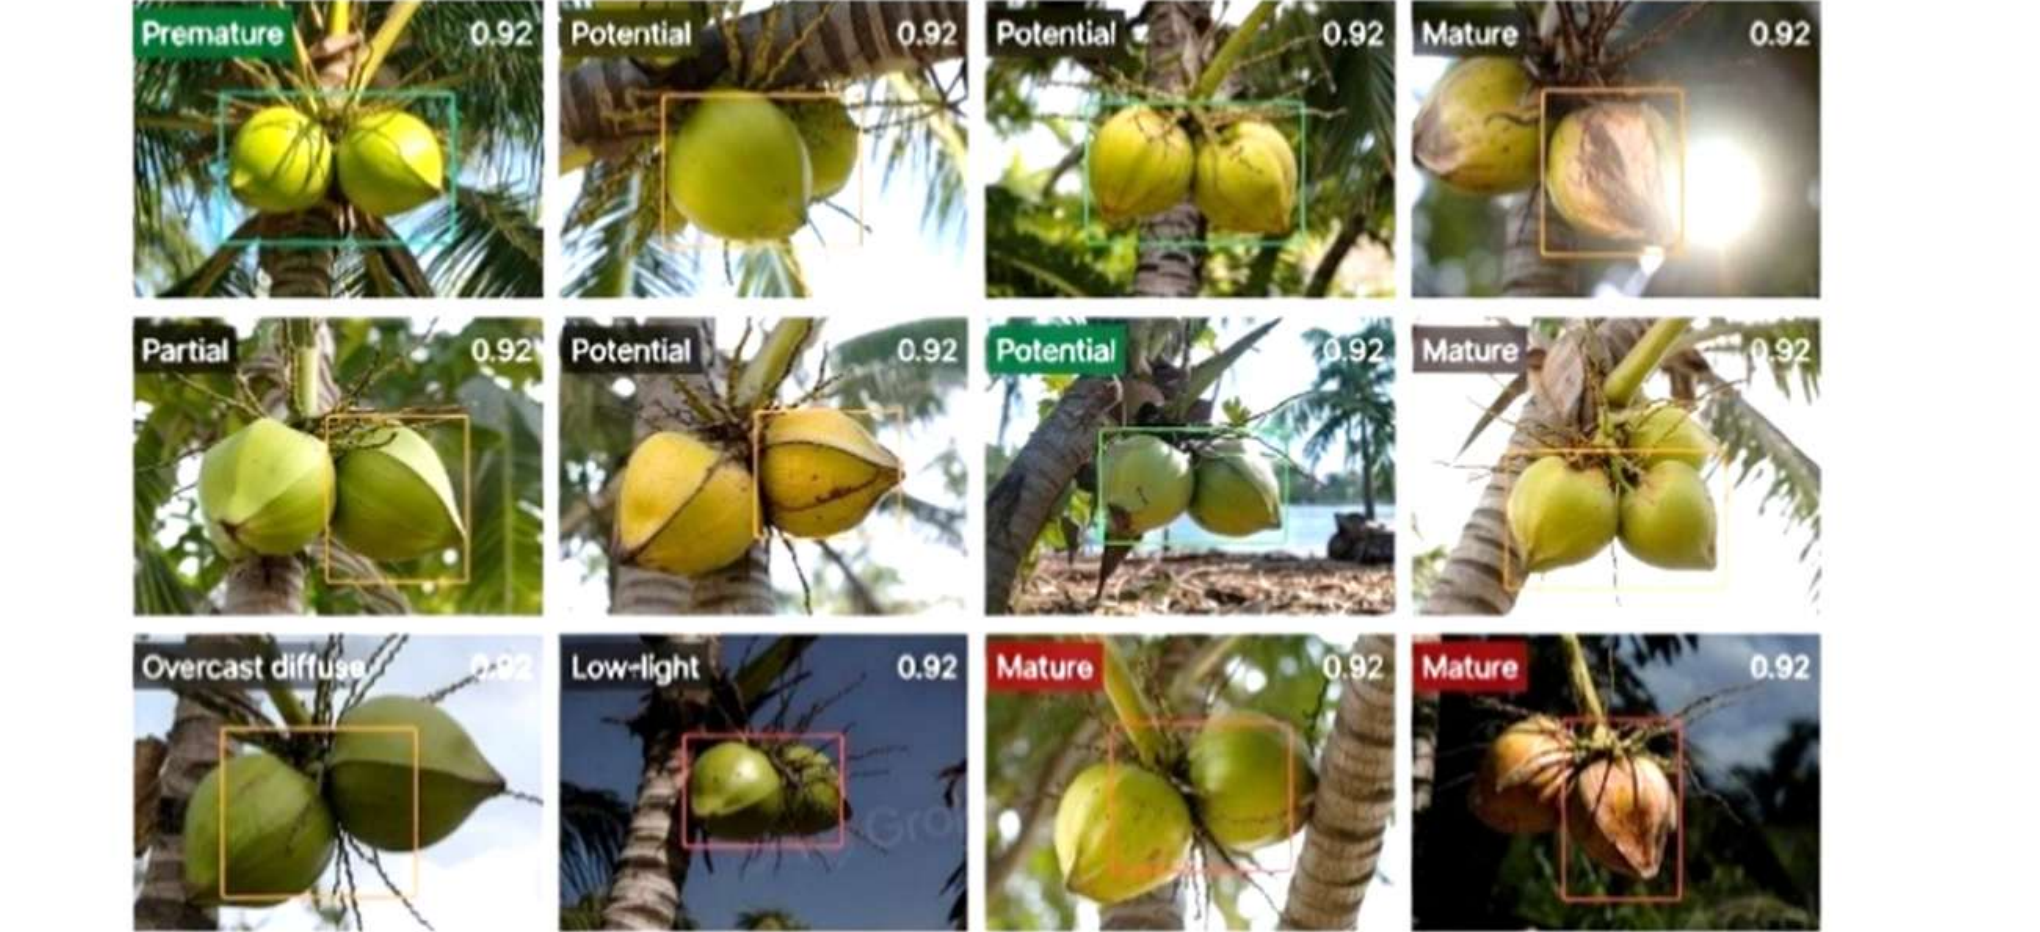
\includegraphics[width=0.95\textwidth]{figures/fig_dataset_samples.png}
\figcap{Figure 4: Sample images and bounding-box annotations from the public coconut datasets (Roboflow previews), showing examples of the tree and ripeness labels. The variation in lighting and viewpoint across these samples is why lighting conditions appear in the limitations.}
\end{figure}

Second, the backend logic that does not depend on the weights was evaluated with a reproducible script (experiments.py, fixed random seeds, run against the project's own modules). It covers: E1, determinism of the engine over 100 random missions of 3 to 12 trees, comparing SHA-256 hashes of the full event and state trace across two runs; E2, routing quality of the nearest-neighbour planner against the exact optimum (5 to 8 trees, 100 instances each) and against a 2-opt reference (10 to 100 trees); E3, exhaustive legality of all 64 ordered state pairs; E4, engine invariants and battery diversion; E5, boustrophedon order for 16 grid and origin configurations; E6, tree matching under re-survey position error using the real matching code on a SQLite database; and E7, engine throughput. Tree positions in E1 to E4 and E7 are random on a $4100\times4100$ farm-pixel field with the dock at the origin, and E6 uses 60 synthetic trees at least 8 m apart. These are simulation experiments and not field measurements.

% ================= RESULTS AND DISCUSSION =================
\irjsec{RESULTS AND DISCUSSION}
\irjsub{A. Detector configuration and accuracy}

\begin{table}[!ht]
\vspace{-2pt}
\tablecap{Table 1. Detector training and inference configuration (all values from the checkpoints' recorded training configuration)}

\centering
\small
\begin{tabular}{|p{0.19\textwidth}|p{0.345\textwidth}|p{0.345\textwidth}|}
\hline
\textbf{Setting} & \textbf{Tree detector} & \textbf{Ripeness detector} \\
\hline
Classes & tree (1) & Mature, Potential, Premature (3) \\
\hline
Dataset & Public tree dataset (Roboflow, CC BY 4.0) & Public maturity dataset (Roboflow, CC BY 4.0) \\
\hline
Base weights & COCO-pretrained YOLOv8n & COCO-pretrained YOLOv8n \\
\hline
Parameters & 3,011,000 (6.2 MB weights) & 3,011,400 (6.2 MB weights) \\
\hline
Epochs & 50 & 50 \\
\hline
Image size & 640 px & 640 px \\
\hline
Batch size & 16 & 16 \\
\hline
Optimizer & auto (Ultralytics default) & auto (Ultralytics default) \\
\hline
Learning rate & lr0 0.01, lrf 0.01 & lr0 0.01, lrf 0.01 \\
\hline
Momentum / weight decay & 0.937 / 0.0005 & 0.937 / 0.0005 \\
\hline
Warm-up epochs & 3 & 3 \\
\hline
Loss gains & box 7.5, cls 0.5, dfl 1.5 & box 7.5, cls 0.5, dfl 1.5 \\
\hline
Augmentation & Ultralytics defaults: HSV colour jitter, scale and translate jitter, horizontal flip, mosaic & Ultralytics defaults: HSV colour jitter, scale and translate jitter, horizontal flip, mosaic \\
\hline
Training hardware & Authors' local machine & Authors' local machine \\
\hline
Inference confidence & 0.40 & 0.25 \\
\hline
Metric IoU & 0.5 and 0.5:0.95 & 0.5 and 0.5:0.95 \\
\hline
\end{tabular}
\end{table}

\begin{table}[!ht]
\vspace{-2pt}
\tablecap{Table 2. Detection accuracy on each model's held-out validation split}

\centering
\small
\begin{tabular}{|l|r|r|r|r|}
\hline
\textbf{Model / class} & \textbf{Precision} & \textbf{Recall} & \textbf{mAP@0.5} & \textbf{mAP@0.5:0.95} \\
\hline
Tree detector & 0.841 & 0.843 & 0.877 & 0.539 \\
\hline
Ripeness: all classes & 0.760 & 0.747 & 0.783 & 0.587 \\
\hline
Ripeness: Mature & 0.637 & 0.607 & 0.631 & 0.430 \\
\hline
Ripeness: Potential & 0.794 & 0.791 & 0.860 & 0.715 \\
\hline
Ripeness: Premature & 0.848 & 0.842 & 0.858 & 0.617 \\
\hline
\end{tabular}
\end{table}

The two detectors reach competitive accuracy on their held-out validation splits: 0.841 precision and 0.877 mAP@0.5 for the tree detector, and an average of 0.760 precision and 0.783 mAP@0.5 for the three ripeness classes. The confusion matrices (Fig.~5) show that most ripeness errors are missed detections (boxes predicted as background, 30 to 35 percent of ground-truth coconuts) rather than cross-class swaps, and the tree detector likewise reports no background region as a tree. The precision-recall curves of both models are shown in Fig.~6.

The structure of the errors is consistent with the class composition of the validation data. The ripeness split contains 971 Premature, 632 Potential and 346 Mature instances, so Mature is both the least represented and the least visually distinct class: a partly turned coconut closely resembles a Potential one. The confusion matrix reflects this, allocating Mature's errors between missed detections and a small number of Potential swaps, which is why Mature's precision (0.637) and recall (0.607) trail the other two classes, while Potential and Premature, with more training instances and more distinct colour cues, reach 0.860 and 0.858 mAP@0.5. Missed detections also dominate the overall error budget: closing that gap, for example with higher input resolution or more inspection images captured per tree, is more promising than refining class decision boundaries. The tree detector performs its easier task by construction: one class of large, high-contrast, isolated targets in top-down imagery, which yields a clean diagonal with no background false positives. A further reason for the absolute level of both scores is the detectors' architecture: because YOLOv8's anchor-free detection strategy predicts each box directly from a single point and its decoupled head aggregates features across scales (the C2f-style fusion), localization remains stable for coconuts of very different apparent sizes and under the illumination variation present in both datasets [2]. Both models work from the same pretrained YOLOv8n base because this lightweight variant matches the target's small search space: adequate localization quality at a scale trainable from scratch on a few thousand images without overfitting.

\begin{figure}[!ht]
\centering
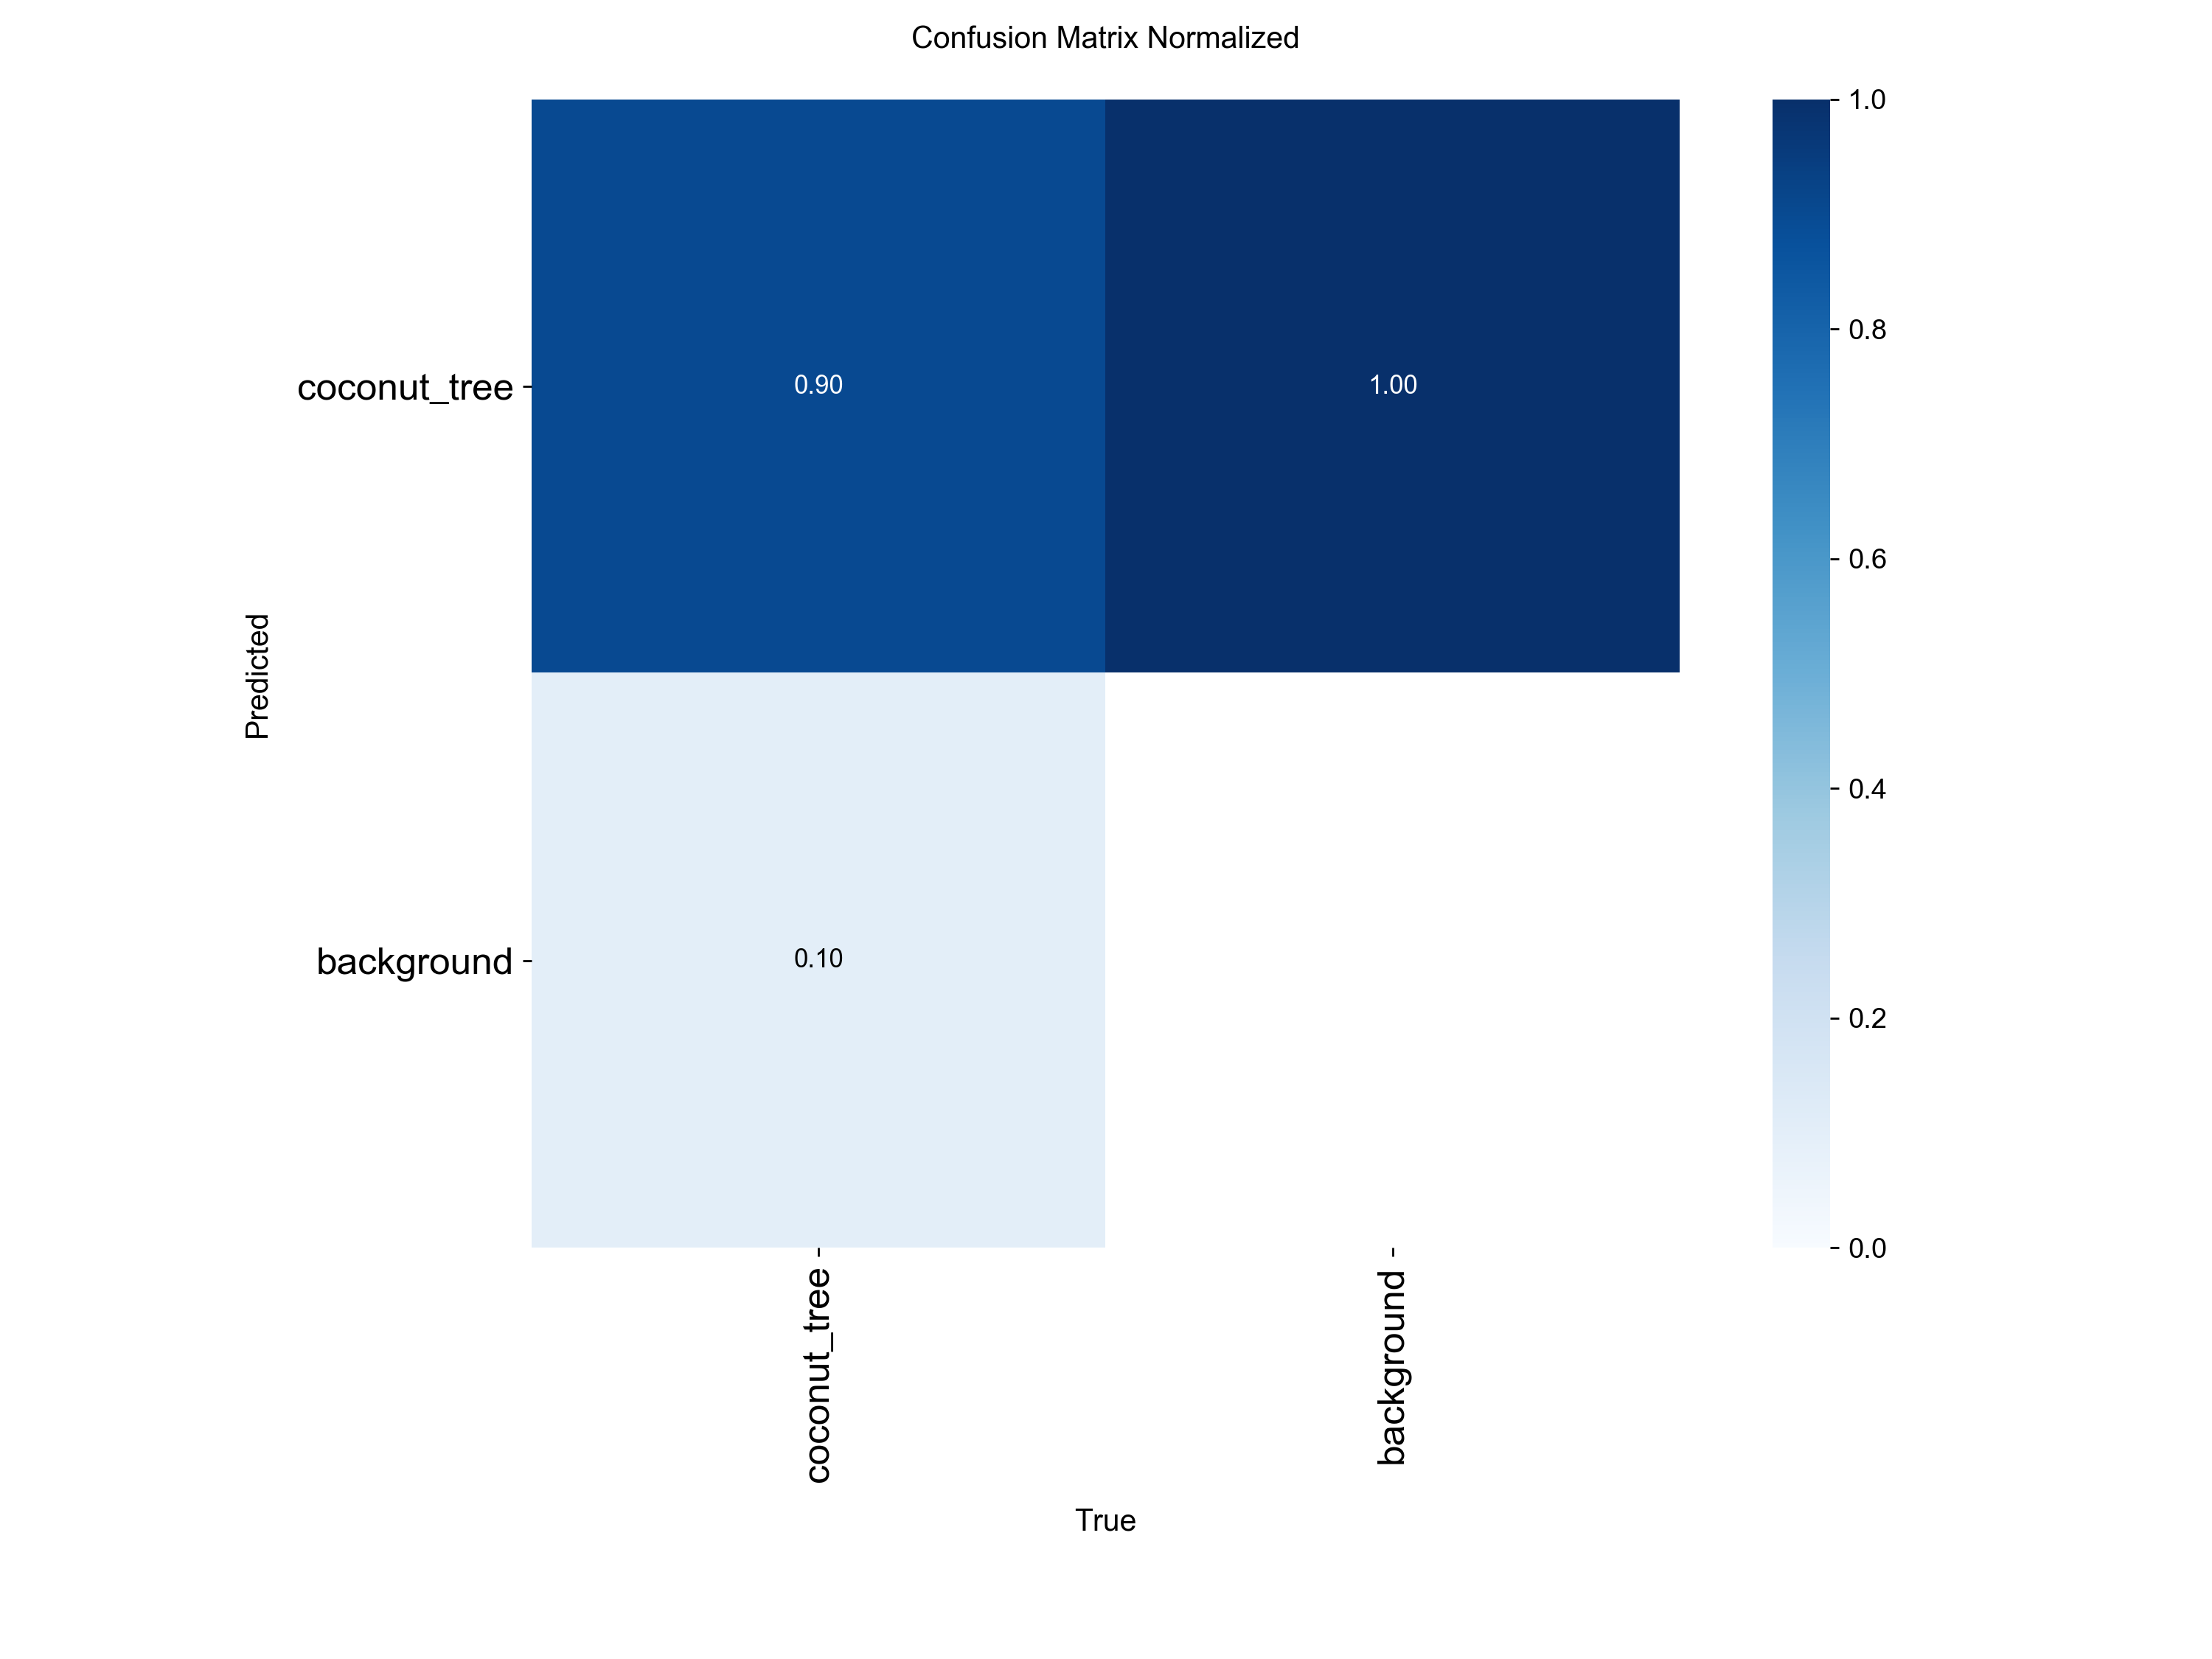
\includegraphics[width=0.45\textwidth]{figures/cmat_tree.png}\hfill
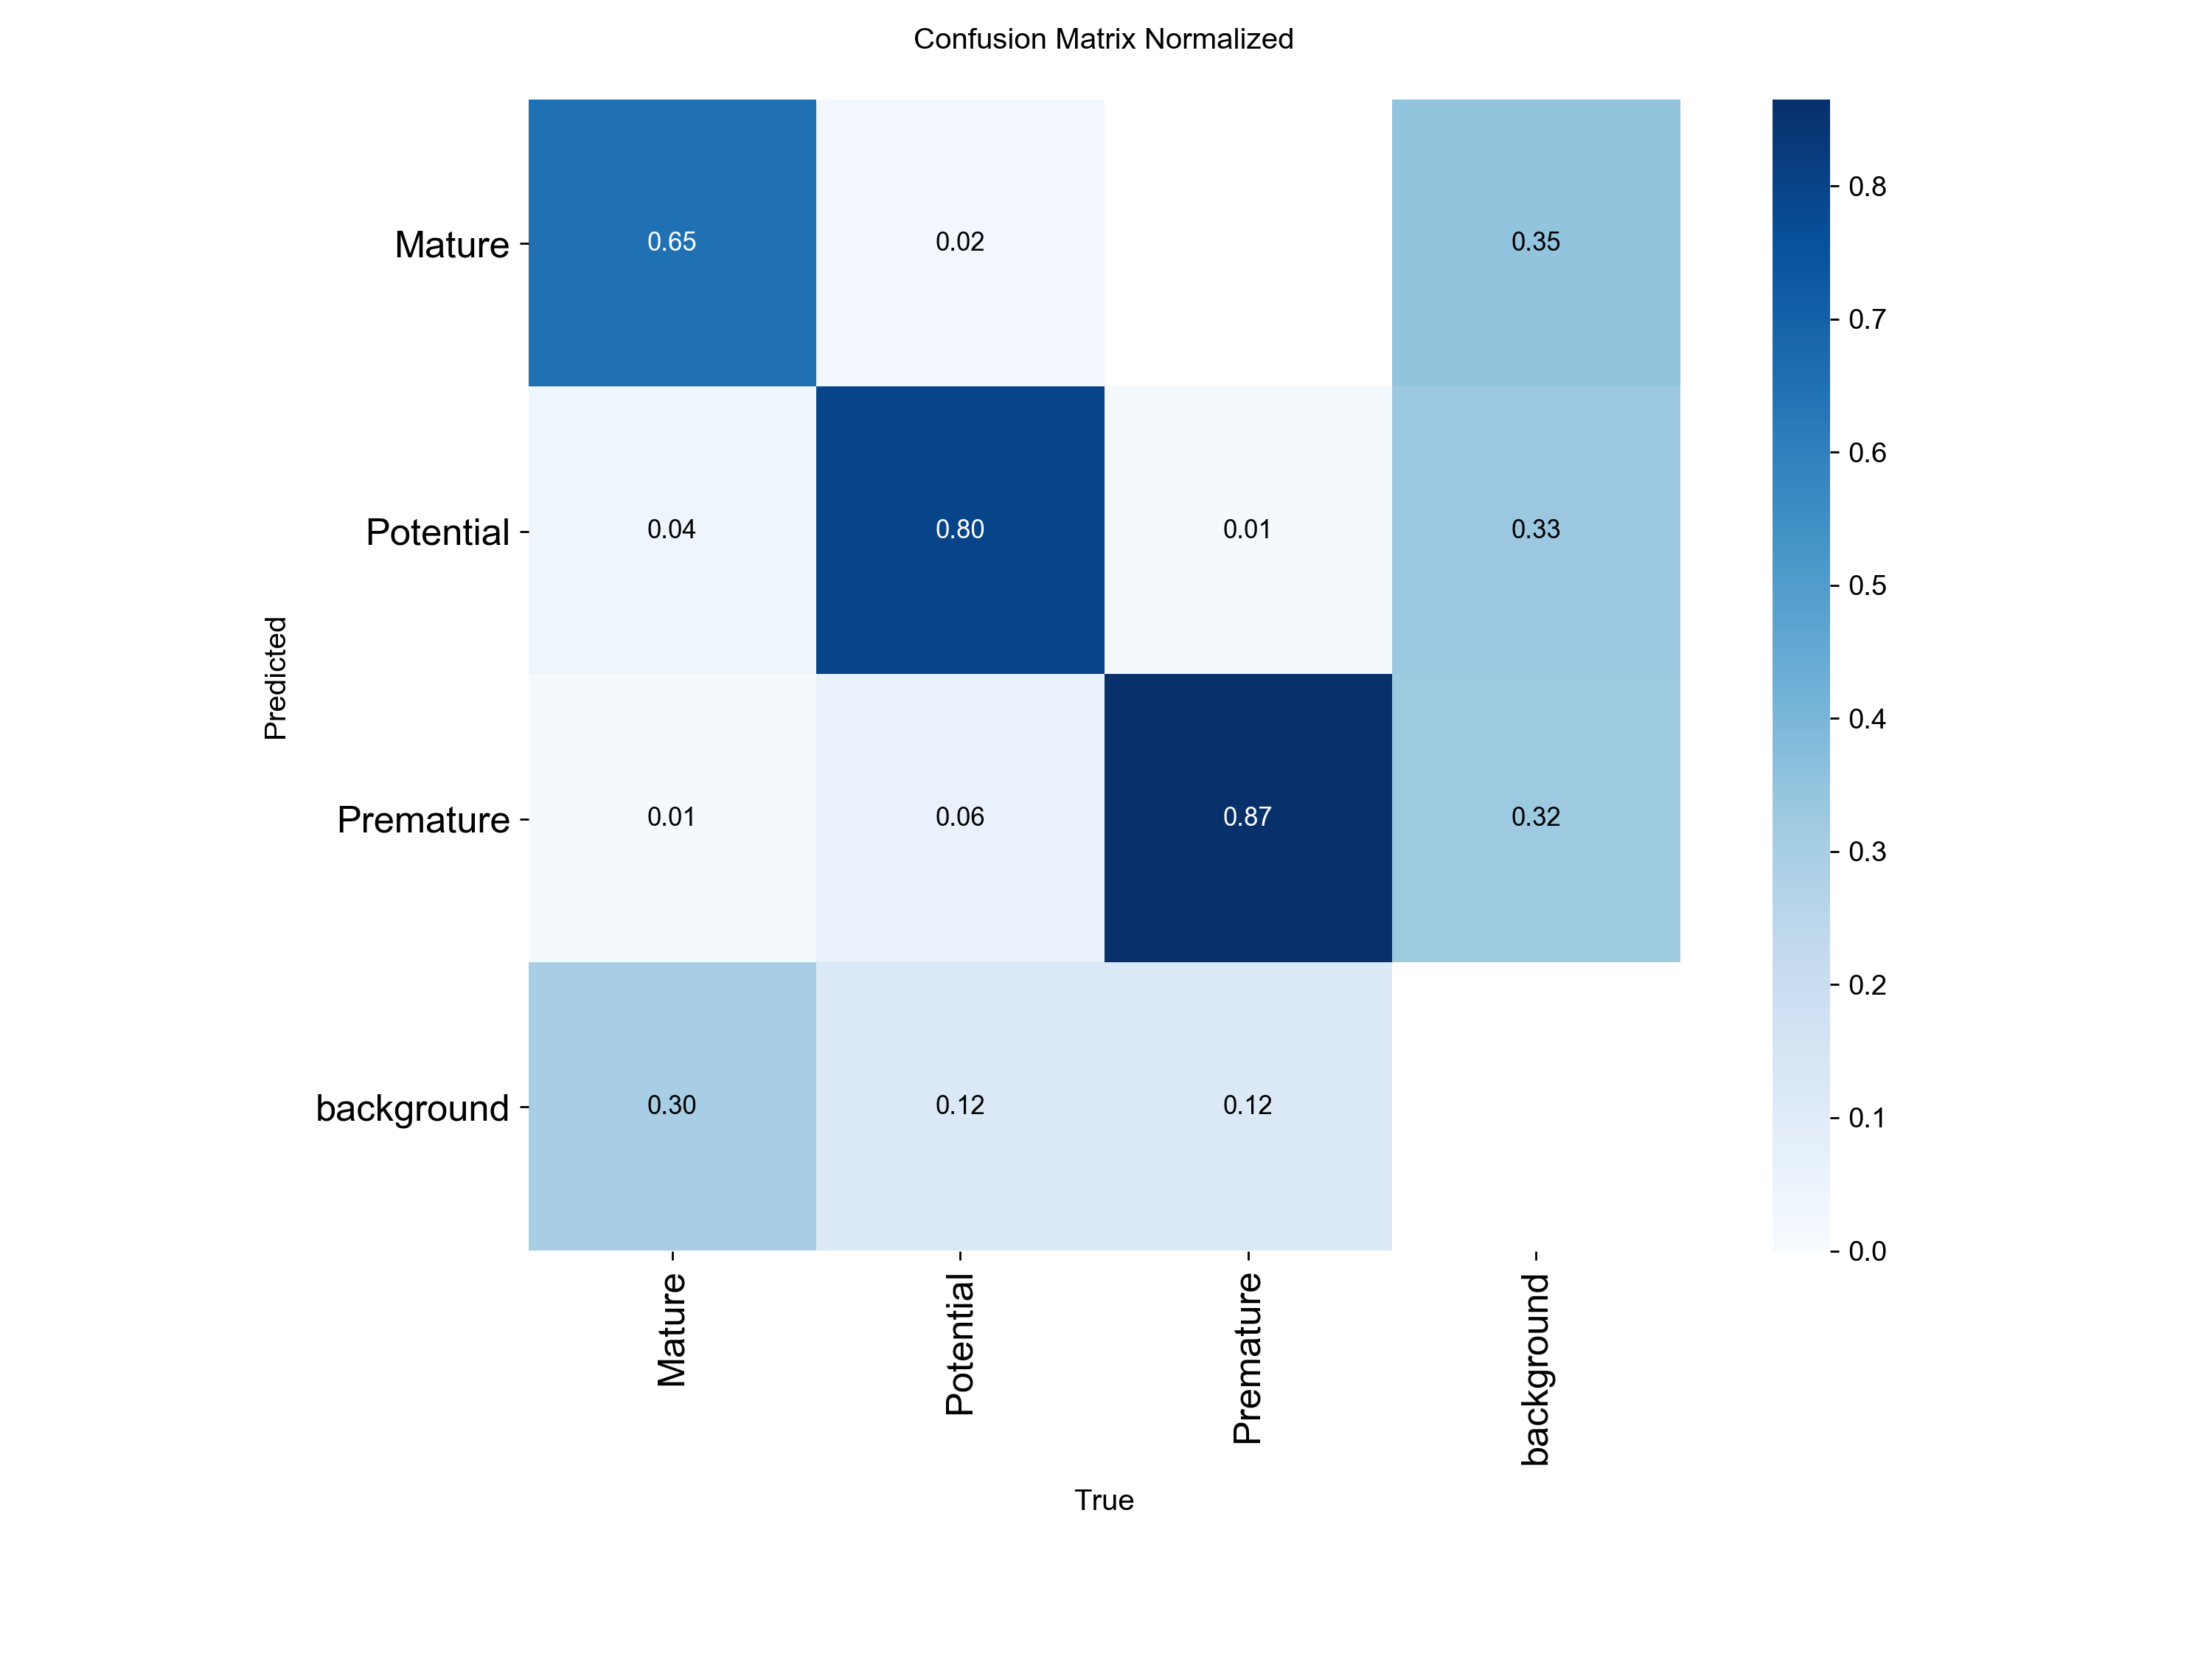
\includegraphics[width=0.45\textwidth]{figures/cmat_coconut.png}
\figcap{Figure 5: Normalised confusion matrices on the held-out validation splits: (left) tree detector, 90 percent diagonal mass with no background false positives; (right) ripeness detector, where most off-diagonal mass lies in the background column (missed detections).}
\end{figure}

\begin{figure}[!ht]
\centering
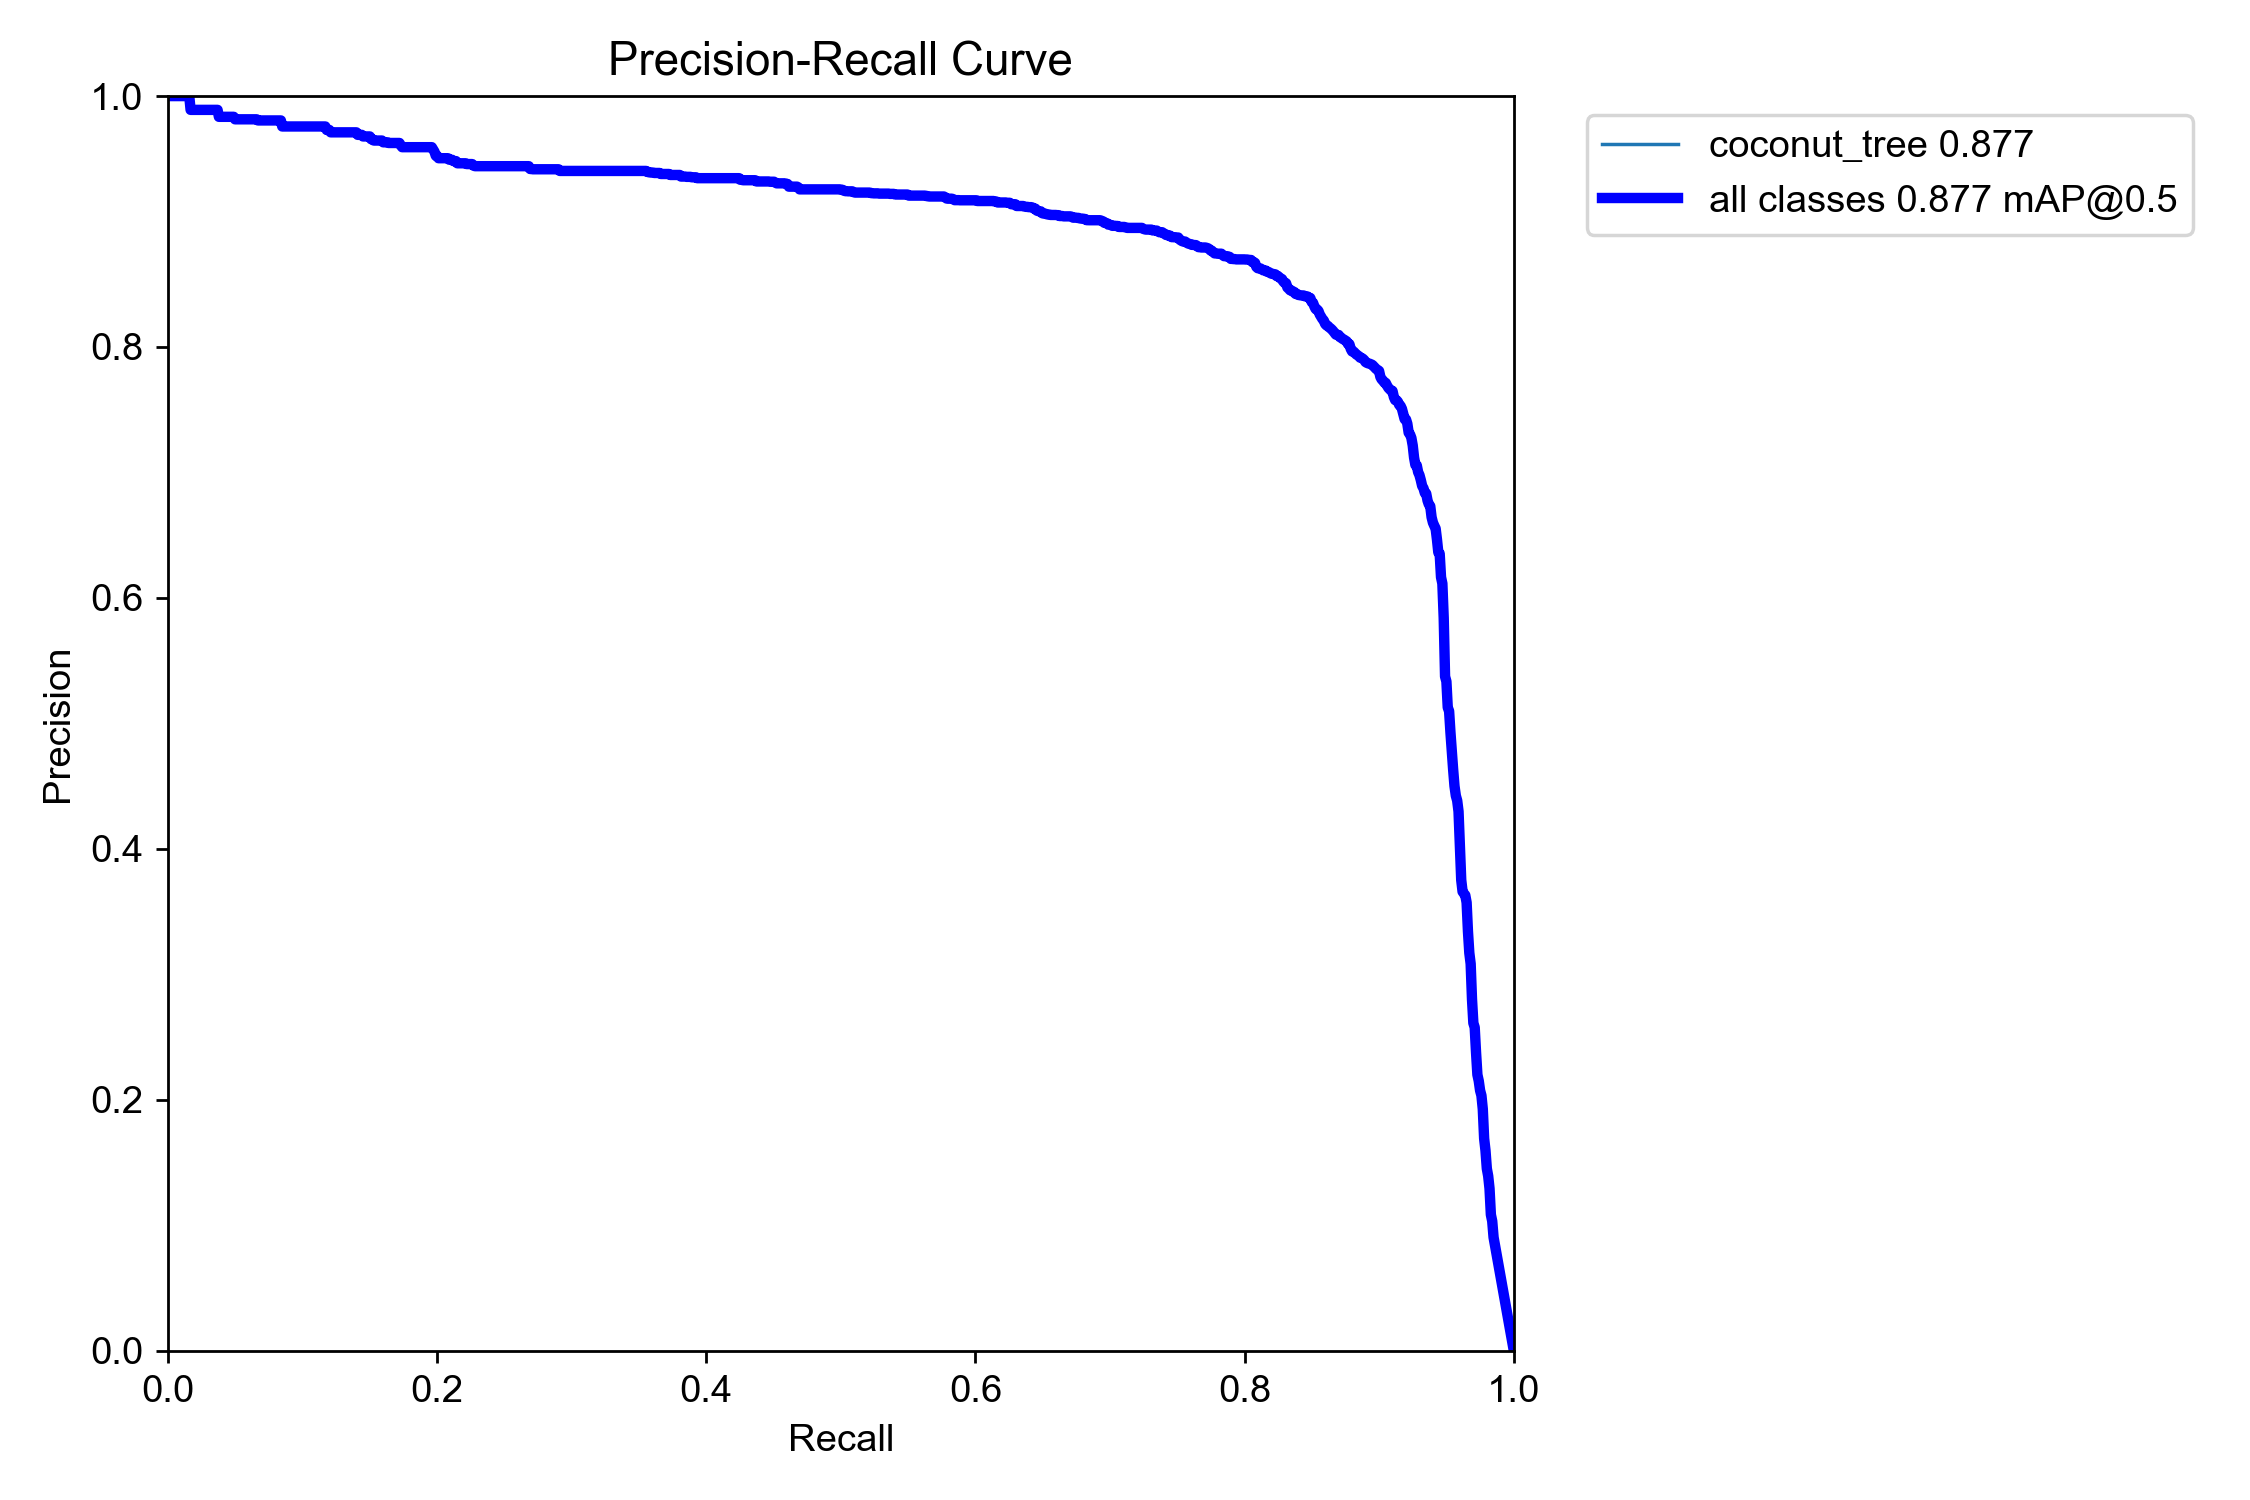
\includegraphics[width=0.45\textwidth]{figures/pr_tree.png}\hfill
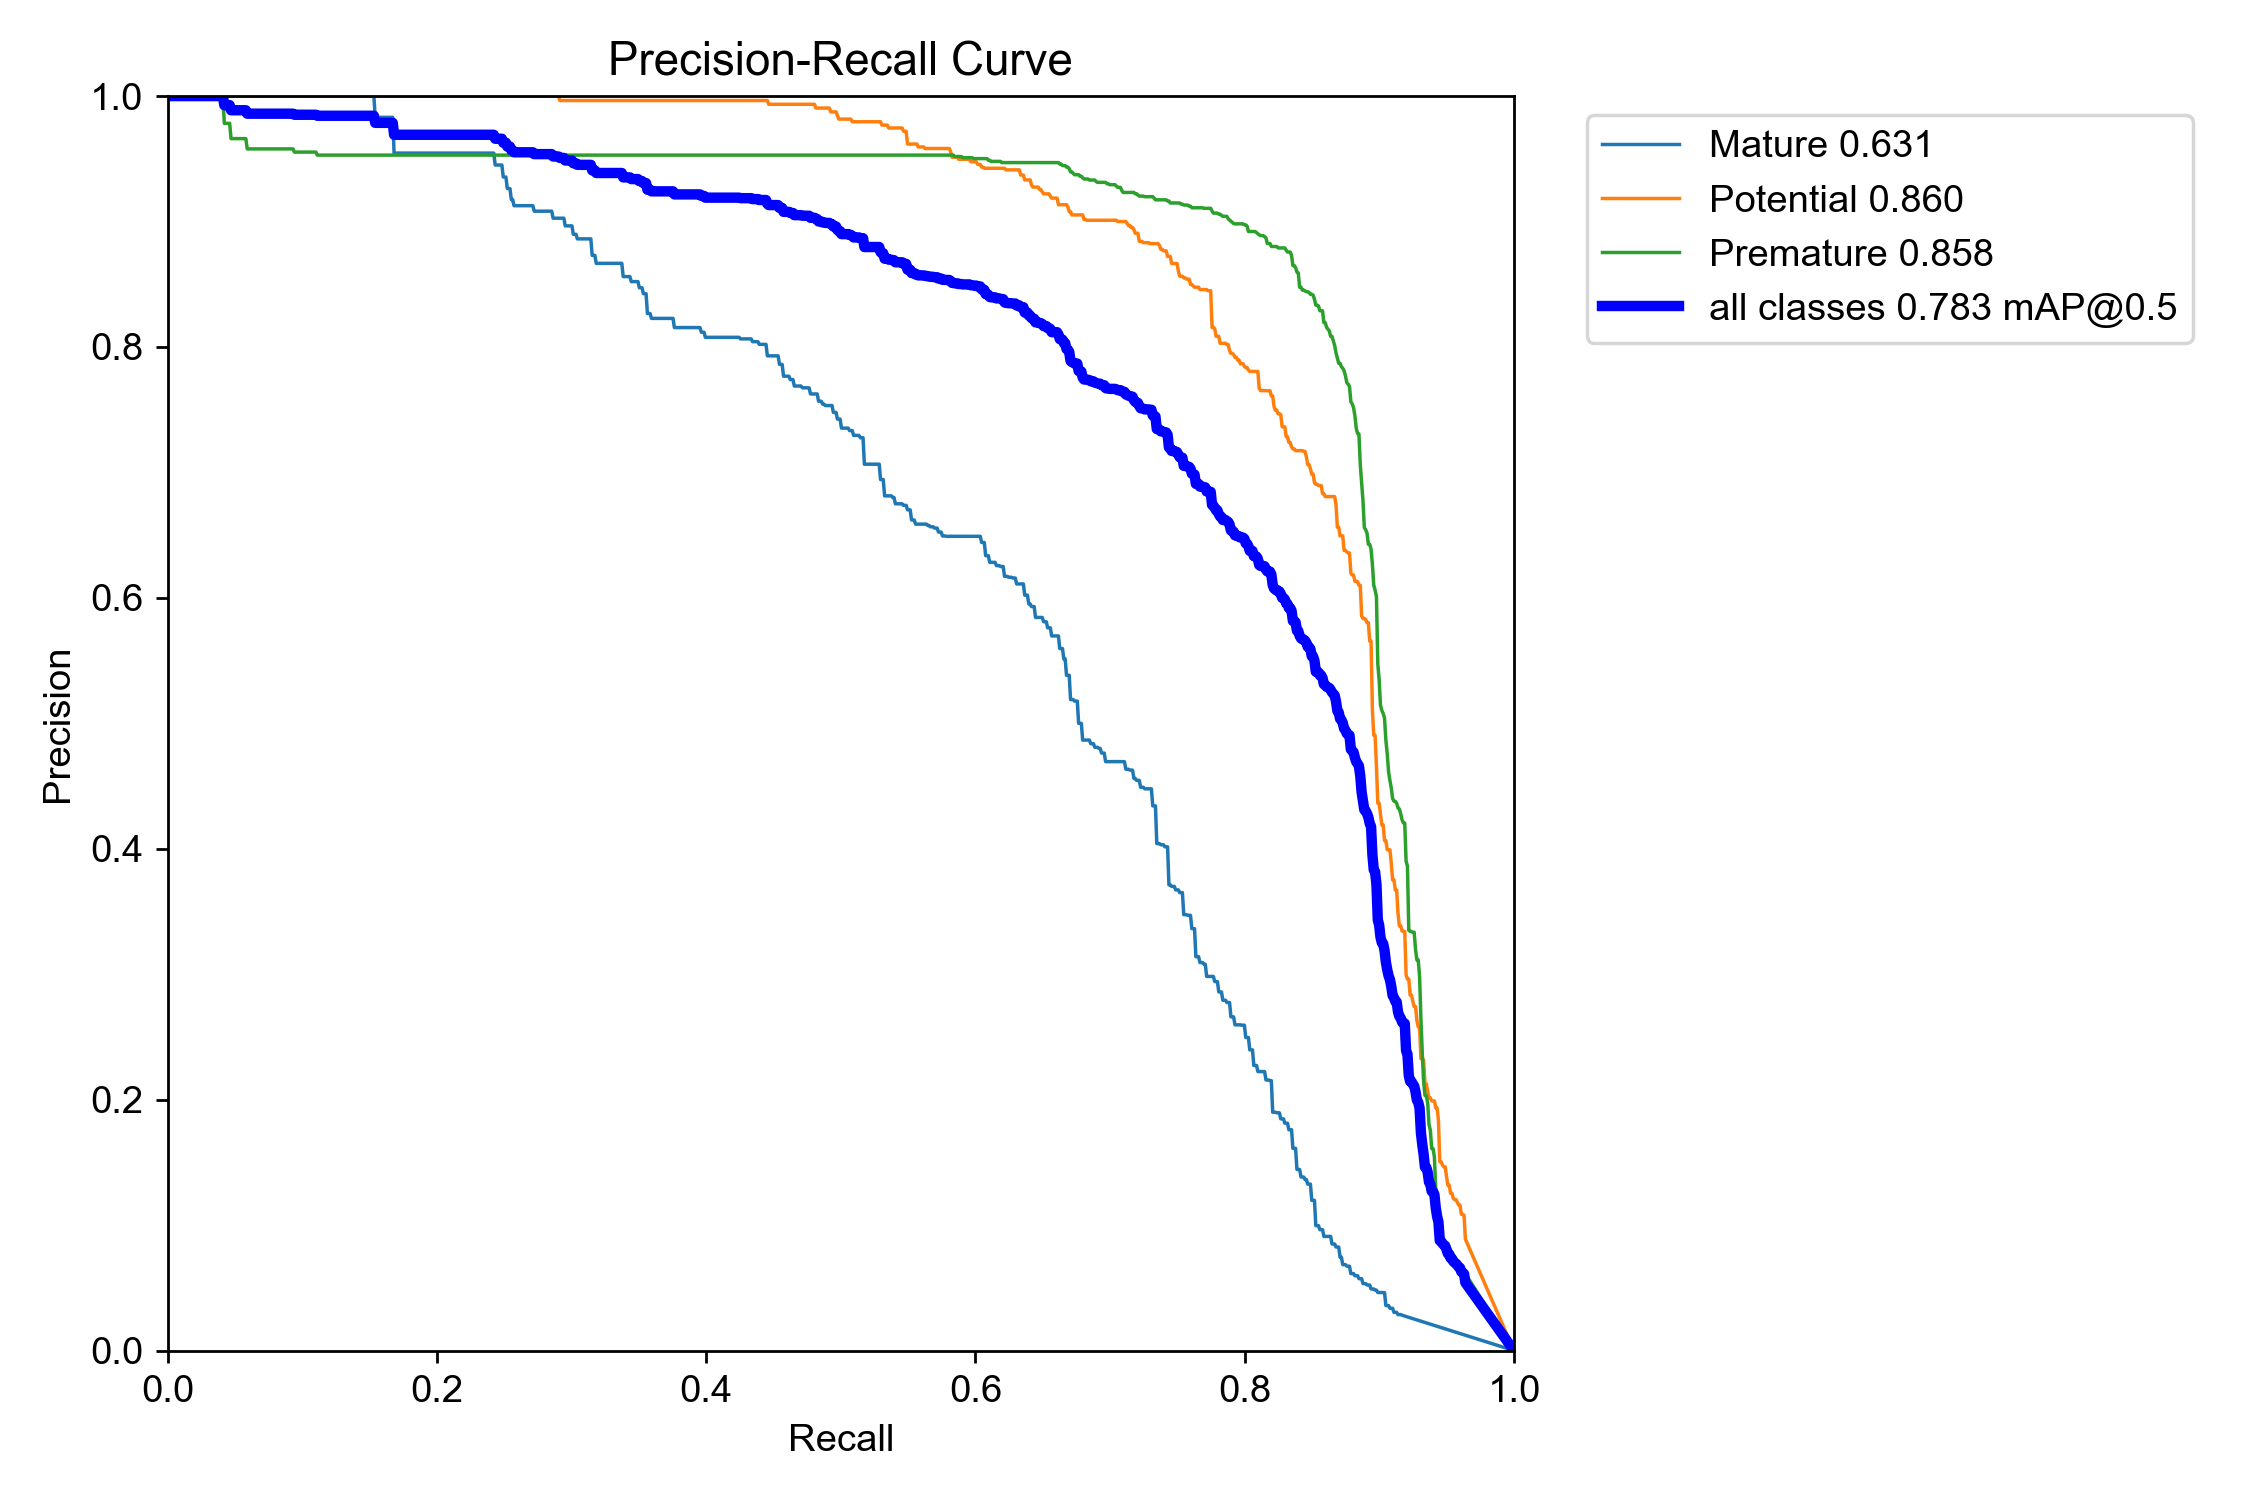
\includegraphics[width=0.45\textwidth]{figures/pr_coconut.png}
\figcap{Figure 6: Precision-recall curves on the held-out validation splits. (Left) tree detector, AP 0.877 at IoU 0.5. (Right) ripeness detector per class: Potential 0.860, Premature 0.858, Mature 0.631 — Mature trails because it is the least represented class and visually resembles Potential.}
\end{figure}

\irjsub{B. End-to-end functional run}
Accuracy alone does not show whether the pieces work together, so a full workflow was executed on a freshly reset database and recorded during the final audit: eight survey images produced eight tiles and 243 tree detections, which became 243 permanent trees; re-running matching reused the existing trees instead of creating duplicates. The one-to-one correspondence is not a coincidence: because the planner positions tiles on a fixed grid and each tree's detections fall on exactly one tile, every detection contributes to exactly one permanent tree. One inspected tree yielded 32 detected coconuts (3 Mature, 2 Potential, 27 Premature) and an inventory snapshot. A harvest mission for one eligible tree with three expected coconuts was started, the simulated robot navigated, harvested three coconuts and returned to the dock, the mission completed, and a run record with timeline, per-tree activity and log was produced. Over the WebSocket, two simultaneous clients received frames, the number of telemetry rows matched the number of frames for the run, and a disconnecting client did not stop the run.

\irjsub{C. Determinism and state-machine correctness}

\begin{table}[!ht]
\vspace{-2pt}
\tablecap{Table 3. Simulation engine and state machine checks}

\centering
\small
\begin{tabular}{|p{0.62\textwidth}|p{0.25\textwidth}|}
\hline
\textbf{Check} & \textbf{Result} \\
\hline
E1: identical event and state trace over two runs (random missions) & 100 / 100 \\
\hline
E3: legal / illegal ordered state pairs & 17 / 47 of 64 \\
\hline
E3: self-transitions allowed & 0 \\
\hline
E3: operational states that can fault to Error & 7 of 7 \\
\hline
E4: illegal transitions attempted by the engine & 0 in 100 missions \\
\hline
E4: missions ending finished and Docked & 100 / 100 \\
\hline
E4: missions with non-increasing battery & 100 / 100 \\
\hline
E4: missions harvesting every tree (others diverted by low battery) & 88 / 100 \\
\hline
E4: mean state transitions per tree & 4.4 \\
\hline
Battery drain at default $60\times$ speed & 1.0\% per real second \\
\hline
\end{tabular}
\end{table}

The engine produced byte-identical traces in every trial. This happens by construction: step(dt) is a pure function with no clock, database or randomness, and the fixed random seeds drive every randomised decision, so the deterministic replay property is what allows runs to be regression-tested without a clock. The engine never requested an illegal transition because every request passed through the transition table. In the stress test at the lowest speed (1 farm-pixel per simulated second) with 10 to 40 trees, the low-battery rule triggered in all four cases and the robot ended Docked, but with the battery at 0.0 percent each time (Table 4 shows the harvested counts). The fixed 20 percent threshold therefore does not guarantee arrival with reserve when the dock is far away, and a distance-aware return threshold is an obvious improvement.

\begin{table}[!ht]
\vspace{-2pt}
\tablecap{Table 4. Battery-low diversion stress test (speed 1.0 px per simulated second)}

\centering
\small
\begin{tabular}{|r|r|r|l|r|}
\hline
\textbf{Trees} & \textbf{Plan length (px)} & \textbf{Harvested} & \textbf{Final state} & \textbf{Final battery (\%)} \\
\hline
10 & 29,935 & 2 & DOCKED & 0.0 \\
\hline
20 & 36,815 & 2 & DOCKED & 0.0 \\
\hline
30 & 72,290 & 1 & DOCKED & 0.0 \\
\hline
40 & 90,398 & 1 & DOCKED & 0.0 \\
\hline
\end{tabular}
\end{table}

\irjsub{D. Routing quality}

\begin{table}[!ht]
\vspace{-2pt}
\tablecap{Table 5. Nearest-neighbour tour length (round trip from the dock)}

\centering
\small
\begin{tabular}{|r|l|r|r|l|}
\hline
\textbf{Trees} & \textbf{Reference} & \textbf{NN excess mean (\%)} & \textbf{NN excess max (\%)} & \textbf{Random order} \\
\hline
5 & exact optimum & 5.56 & 20.89 & $1.33\times$ \\
\hline
6 & exact optimum & 5.92 & 28.79 & $1.47\times$ \\
\hline
7 & exact optimum & 8.63 & 30.31 & $1.55\times$ \\
\hline
8 & exact optimum & 9.24 & 28.02 & $1.66\times$ \\
\hline
10 & 2-opt reference & 10.14 & -- & $1.72\times$ (vs NN) \\
\hline
20 & 2-opt reference & 14.42 & -- & $2.28\times$ (vs NN) \\
\hline
50 & 2-opt reference & 15.0 & -- & $3.83\times$ (vs NN) \\
\hline
100 & 2-opt reference & 16.69 & -- & $5.33\times$ (vs NN) \\
\hline
\end{tabular}
\end{table}

\begin{figure}[!ht]
\centering
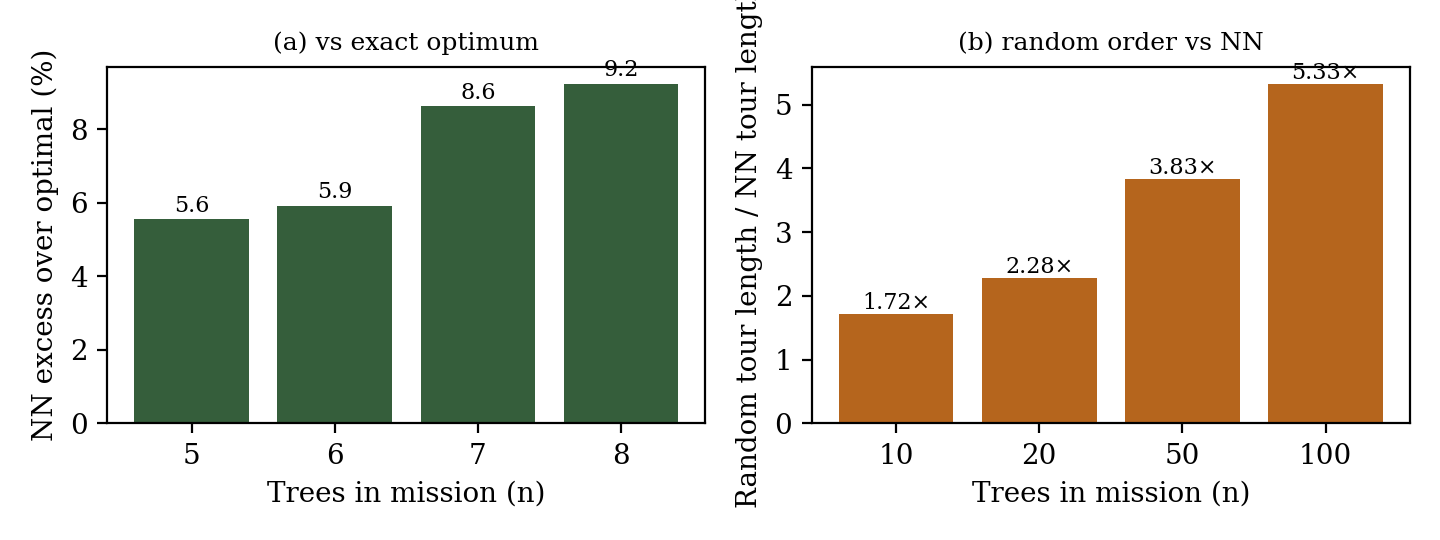
\includegraphics[width=0.95\textwidth]{figures/extracted/image4.png}
\figcap{Figure 7: (a) Excess tour length of nearest neighbour over the exact optimum for 5 to 8 tree missions (mean and worst case): the excess grows as the greedy early decisions accumulate; (b) length of a random visiting order relative to nearest neighbour for 10 to 100 tree missions: without spatial grouping the random order degrades far faster.}
\end{figure}

Nearest neighbour was on average 5.6 to 9.2 percent longer than the exact optimum for 5 to 8 trees, with a worst case of 30.3 percent, and its excess over a 2-opt reference grew from 10.1 percent at 10 trees to 16.7 percent at 100 trees. A random visiting order was 1.7 to 5.3 times longer than nearest neighbour as missions grew. The growth pattern in Fig.~7 is explained by how greedy selection works: nearest neighbour always takes the locally closest stop, which is near-optimal while early choices are cheap, but every early decision is locked in, so as the tour grows the accumulated cost of those irreversible early excursions rises, which is exactly the behaviour the Rosenkrantz bound analysis [6] predicts. The random order degrades far faster because it carries no spatial grouping at all — each hop ignores the clustering of the previous one. Nearest neighbour is therefore a sound first choice: it is explainable, deterministic and far better than an unordered visit, but a 2-opt pass would remove a further 10 to 17 percent of travel and is a low-cost extension.

\irjsub{E. Tree matching under re-survey error}

\begin{table}[!ht]
\vspace{-2pt}
\tablecap{Table 6. Re-survey matching with 60 trees spaced at least 8 m apart}

\centering
\small
\begin{tabular}{|r|r|r|r|r|}
\hline
\textbf{Error (px)} & \textbf{Error (m, per axis)} & \textbf{Trees after survey 1} & \textbf{Trees after re-survey} & \textbf{Duplicates} \\
\hline
0 & 0.0 & 60 & 60 & 0 \\
\hline
10 & 0.54 & 60 & 60 & 0 \\
\hline
20 & 1.09 & 60 & 60 & 0 \\
\hline
40 & 2.17 & 60 & 71 & 11 \\
\hline
80 & 4.34 & 60 & 79 & 19 \\
\hline
\end{tabular}
\end{table}

\begin{figure}[!ht]
\centering
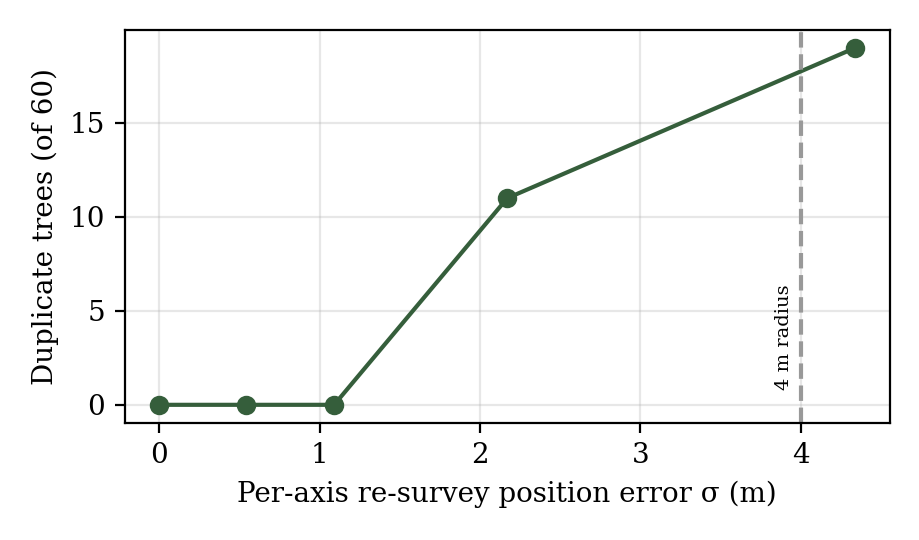
\includegraphics[width=0.55\textwidth]{figures/extracted/image5.png}
\figcap{Figure 8: Duplicate trees created by the 4 m matching radius when a re-survey displaces tree positions (per-axis error in pixels and metres); 0 duplicates up to 1.09 m, 11 at 2.17 m, 19 at 4.34 m.}
\end{figure}

Survey 1 produced exactly the 60 true trees (no false merges), and a re-survey with per-axis error up to about 1.1 m created no duplicates. At 2.2 m and 4.3 m the rule created 11 and 19 duplicates, which matches what a fixed 4 m radius implies for a two-dimensional Gaussian error: as the per-axis error grows, an increasing fraction of re-sampled positions lands farther than 4 m from the original tree, so the probability that a displacement breaks the merge radius rises with the error size. The result also exposes the rule's main assumption: trees closer than 4 m are merged. In a preliminary run with trees placed freely at random, 14 of 60 trees were merged for that reason. Coconut palms are normally planted at wider spacing, typically around 7.5 to 9 m [10], so the 4 m radius is suitable for typical plantations but should be reduced for very dense plots.

\irjsub{F. Throughput and engineering observations}
The remaining results measure cost rather than correctness. In our test environment the engine ran at about 114,575 to 119,599 one-second steps per second on a single CPU core, more than 800 times the 60 steps per second needed to run in real time at the default $60\times$ speed, so simulation cost is negligible next to database round-trips. The latter dominated the deployed system: the managed serverless PostgreSQL adds a round-trip floor of roughly 2 s per request, a batched update of 302 rows took about 80 s, and replacing a per-tree query loop (about 600 sequential queries) with two grouped aggregates reduced the tree-summary endpoint from a hang beyond 20 s to about 3 s. These observations are from the development log of the project and were not measured under a controlled benchmark.

% ================= LIMITATIONS =================
\irjsec{LIMITATIONS AND FUTURE WORK}
The robot is simulated and no physical climbing hardware has been integrated, so mechanical grasping, trunk climbing and sensing noise are not evaluated. All detector accuracy comes from public datasets captured under conditions we do not control: the images include daylight and mixed weather but no night-time or irrigation-dusk footage, accuracy may drop on locally captured plantation imagery, and the ripeness validation split is small (618 images, 1,949 instances). The datasets cover coconut palms only, so the tree detector would not transfer to other plantation species without retraining and new labels. GPS positions are generated from a base coordinate and the tile grid rather than read from real geotags, which means absolute positions are synthetic although relative geometry is consistent; the matching radius also assumes palms are planted further apart than 4 m, which is typical for coconut [10] but not guaranteed for every plot, and real GPS error will add measurement noise on top of the simulation study in Table 6. The routing experiments use random positions rather than surveyed plantations, so tour-length conclusions are indicative rather than field measurements. The system supports one farm and one robot, has no authentication, and renders tree overlays with DOM elements, which performs well at about 300 trees but will need canvas rendering or stronger culling for thousands.

Future work includes field validation of both detectors on locally captured images, real geotagging and RTK positions, a distance-aware battery return rule, 2-opt route refinement, post-harvest verification scans, multi-robot and multi-farm support, and replacing the simulation engine with a physical robot that satisfies the same telemetry and command contract.

% ================= CONCLUSION =================
\irjsec{CONCLUSION}
Veraxis shows that a plantation can be treated as a persistent digital asset: drone tiles become permanent, deduplicated trees; close-up scans become immutable inventory; and a planner turns inventory into a reproducible harvest mission executed by a robot whose behaviour is owned entirely by the backend. Separating tree detection from ripeness inspection, and route planning from movement planning and execution, keeps both layers independently replaceable: either detector or the entire simulated robot can be swapped without touching the rest. The experiments confirm deterministic simulation, a respected state machine, nearest-neighbour routing that is acceptable but improvable, and duplicate-free matching for re-survey errors up to about 1 m. Future work will focus on large-scale field validation, multi-camera close-up perception for the inspection pass, adaptive harvesting strategies under varying environmental conditions, and the physical integration of the climbing robot.

% ================= ACKNOWLEDGEMENTS =================
\irjsec{ACKNOWLEDGEMENTS}
The authors thank their project guide Dr.~Madhu B.K, the Department of Computer Science and Engineering and the management of Vidya Vikas Institute of Engineering and Technology Mysuru for their guidance and support.

% ================= REFERENCES =================
\needspace{5\baselineskip}
\irjsec{REFERENCES}
\begin{thebibliography}{10}
\setlength{\itemsep}{1pt}
\bibitem{redmon} J. Redmon, S. Divvala, R. Girshick and A. Farhadi, ``You Only Look Once: Unified, Real-Time Object Detection,'' Proc. IEEE Conf. on Computer Vision and Pattern Recognition (CVPR), 2016, pp. 779--788.
\bibitem{jocher} G. Jocher, A. Chaurasia and J. Qiu, ``Ultralytics YOLOv8,'' 2023. [Online]. Available: \url{https://github.com/ultralytics/ultralytics}
\bibitem{koirala} A. Koirala, K. B. Walsh, Z. Wang and C. McCarthy, ``Deep learning for real-time fruit detection and orchard fruit load estimation: benchmarking of MangoYOLO,'' Precision Agriculture, vol. 20, no. 6, pp. 1107--1135, 2019.
\bibitem{bargoti} S. Bargoti and J. Underwood, ``Deep fruit detection in orchards,'' Proc. IEEE Int. Conf. on Robotics and Automation (ICRA), 2017, pp. 3626--3633.
\bibitem{grieves} M. Grieves and J. Vickers, ``Digital Twin: Mitigating Unpredictable, Undesirable Emergent Behavior in Complex Systems,'' in Transdisciplinary Perspectives on Complex Systems, Springer, 2017, pp. 85--113.
\bibitem{rosenkrantz} D. J. Rosenkrantz, R. E. Stearns and P. M. Lewis II, ``An analysis of several heuristics for the traveling salesman problem,'' SIAM Journal on Computing, vol. 6, no. 3, pp. 563--581, 1977.
\bibitem{croes} G. A. Croes, ``A method for solving traveling-salesman problems,'' Operations Research, vol. 6, no. 6, pp. 791--812, 1958.
\bibitem{harel} D. Harel, ``Statecharts: A visual formalism for complex systems,'' Science of Computer Programming, vol. 8, no. 3, pp. 231--274, 1987.
\bibitem{fette} I. Fette and A. Melnikov, ``The WebSocket Protocol,'' RFC 6455, Internet Engineering Task Force, 2011. [Online]. Available: \url{https://datatracker.ietf.org/doc/html/rfc6455}
\bibitem{cpcri} M. K. Nair, ``Coconut Cultivation Practices,'' Indian Council of Agricultural Research -- Central Plantation Crops Research Institute (ICAR-CPCRI), Kasaragod, India, July 1989. [Online]. Available: \url{https://cpcri.gov.in/filemgr/webfs/publication/pamphlet1e_july1989.pdf}
\end{thebibliography}

\end{document}
